\section{Introduction}
Les forêts aléatoire reste jusqu'à aujourd'hui l'un des outils de machine learning les plus populaire vue la précision la robustesse qu'elles nous offres sur de vrai jeux de données, nous allons voir dans ce projet une nouvelle classe des forêts aléatoires: \textbf{'les Forêts de Mondrian"} (MF)
en raison de l'arborescence sous-jacente de chaque classifieur de l'ensemble est un \textbf{processus de Mondrian}.
Nous allons voir dans ce projet les propriétés de ces forêts aléatoires de Mondrian, ainsi que quelque applications à l'aide de Python.


\section{Approche}

Soit $N: (x_1,y_1),\dots,(x_N,y_N)\in \mathbb{R}^D\times \mathcal{Y}$ nos données d'apprentissage (train), l'objectif ici est de prédire $y\in \mathcal{Y}$ pour les points $x\in\mathbb{R}^D$. On va se focaliser sur la classification multi-classes ou $\mathcal{Y}:=\{1, \ldots, K\}$, cependant, il est possible d'étendre la méthodologie à d'autres
tâches d'apprentissage supervisé telles que la régression. Soit $X_{1:n}:=(x_1,\dots,x_n),Y_{1:n}:=(y_1,\dots,y_n)$, et $\mathcal{D}_{1,n}:=(X_{1:n},Y_{1:n})$.

Les Mondrian forests sont construits comme les forets aléatoires:  Soit $\mathcal{D}_{1:N}$ nos données d'apprentissage, on tire un échantillon $T_1,\dots,T_M$ indépendants des arbres Mondrian (que l'on va décrire dans la section 2). La prédiction fait par chaque arbre de Mondrian $T_m$ est une distribution $p_{T_{m}}\left(y \mid x, \mathcal{D}_{1: N}\right)$ de $y$ pour $x$. La prédiction fait par les forets de Mondrian est $\frac{1}{M} \sum_{m=1}^{M} p_{T_{m}}\left(y \mid x, \mathcal{D}_{1: N}\right)$ de l'arbre de prédiction. Quand $M \rightarrow \infty$, cette moyenne vers $\mathbb{E}_{T \sim \operatorname{MT}\left(\lambda, \mathcal{D}_{1: N}\right)}\left[p_{T}\left(y \mid x, \mathcal{D}_{1: N}\right)\right]$ où $MT(\lambda,\mathcal{D}_{1:N})$ est la distribution de l'arbre de Mondrian.
Comme la limite de l'espérance ne dépends pas de $M$, on ne s'attendrait pas à voir un sur ajustement quand $M$ augmente.

Dans le cadre de l'apprentissage en ligne, les exemples de formation sont présentés l'un après l'autre dans une
séquences d'essais. les forêts de Mondrian excelle dans ce cadre la: à l'itération $N+1$, chaque arbre de Mondrian $T \sim \operatorname{MT}\left(\lambda, \mathcal{D}_{1: N}\right)$  est mis à jour pour incorporer l'exemple labellisé suivant: $(x_{N+1},y_{N+1})$  par échantillonnage d'un arbre étendu $T'\prime$ de $\operatorname{MTx}\left(\lambda, T, \mathcal{D}_{N+1}\right)$. En utilisant les propriétés du processus de Mondrian, on peut choisir la probabilité de $\operatorname{MTx}$ avec $T^\prime=T$ sur $\mathcal{D}_{1:N}$ et $T^\prime$ est répartit en fonction de $\operatorname{MT}\left(\lambda, \mathcal{D}_{1: N+1}\right)$:

$$
\begin{aligned}
T & \sim \operatorname{MT}\left(\lambda, \mathcal{D}_{1: N}\right) \\
T^{\prime} \mid T, \mathcal{D}_{1: N+1} & \sim \operatorname{MTx}\left(\lambda, T, \mathcal{D}_{N+1}\right)\\
T^\prime &\sim \operatorname{MT}\left(\lamda,\mathcal{D}_{1:N+1}\right)
\end{aligned}
$$


Par conséquent, la distribution des arbres de Mondrian entraînés sur un ensemble de données de manière incrémentée est identique à celui des arbres Mondrian entraînés sur le même jeu de données de manière groupées , indépendant de l'ordre dans lequel les points de données ont été observés. À notre connaissance, aucun des forêts aléatoires en ligne existantes ont cette propriété.

De plus, nous peut tirer un échantillon de $\operatorname{MTx}\left(\lambda, T, \mathcal{D}_{N+1}\right)$, la complexité évolue avec la profondeur de l'arbre, qui est typiquement logarithmique en $N$ de manière efficace.

En traitant le paramètre en ligne comme une séquence de groupes de plus en plus importants, le problème est généralement un problème de calcule, les forets de Mondrian nous permettent de réaliser efficacement cette approche.

Nous allons définir avec plus de détaille dans la suite:
\begin{itemize}
    \item[$\bullet$] La distribution des arbres de Mondrian $\operatorname{MT}\left(\lambda, \mathcal{D}_{1: N}\right)$
    \item[$\bullet$] l'indexe de distribution $p_{T}\left(y \mid x, \mathcal{D}_{1: N}\right)$
    \item[$\bullet$] La distribution mise a jour $\operatorname{MTx}\left(\lambda, T, \mathcal{D}_{N+1}\right)$
\end{itemize}

\section{Arbres de Mondrian}
Nous allons poser l'hypothèse que ici l'arbre de décision dans $\mathbb{R}^D$ sera hiérarchique, partition binaire de $\mathbb{R}^D$ et une règle pour prédire le label des points de test à partir des données d'apprentissage. La structure de l'arbre de décision est  fini, enraciné, strictement binaire $T$.

Un ensemble fini de noeuds est défini tel que:

\begin{itemize}
    \item[$\bullet$] chaque noeud $j$ a exactement un nœud parent, sauf pour un nœud racine distingué $\epsilon$ qui n'a pas de parents 
    \item[$\bullet$] chaque noeud $j$ est le parent d'exactement zéro ou deux noeuds enfants: (le noeud de gauche "$\operatorname{left}(j)$" et le noeud de droite "$\operatorname{right}(j)$")
\end{itemize}

On note les feuilles de $T$ (les noeuds sans enfants) ("$leaves(T)$") chaque noeud de l'arbre $j\in T$ est associé avec un bloc $B_j\subset\mathbb{R}^D$ de l'ensemble de départ comme suit: 
Aux racines, on a $B_\epsilon=\mathbb{R}^D$, tandis que chaque nœud interne $j\in T \backslash \operatorname{leaves}(T)$ avec deux enfants qui représentent une division du bloc des parent en deux moitiés, avec $\delta_j\in\{1,\dots,D\}$ qui indique la dimension du split et $\xi_{j}$ qui représente la localisation du split, en particulier:

$$
\begin{aligned}
B_{\text {left }(j)}&:=\left\{x \in B_{j}: x_{\delta_{j}} \leq \xi_{j}\right\} \\
\quad B_{\text {right }(j)}&:=\mid\left\{x \in B_{j}: x_{\delta_{j}}>\xi_{j}\right\}
\end{aligned}
$$

On appel $(T,\delta,\xi)$ un arbre de décision. On note que les blocs associaient avec les feuilles de l'arbre forme une partition de $\mathbb{R}^D$, on peut écrire $B_{j}=\left(\ell_{j 1}, u_{j 1}\right] \times \ldots \times\left(\ell_{j D}, u_{j D}\right]$ ou $\ell_{jd}$ et $u_{jd}$ représentent les bornes inférieurs et supérieurs du bloc rectangulaire $B_j$ le long de la dimension $d$. On pose $\ell_{j}=\left\{\ell_{j 1}, \ell_{j 2}, \ldots, \ell_{j D}\right\}$ et $\mathbf{u}_{j}=\left\{u_{j 1}, u_{j 2}, \ldots, u_{j D}\right\}$.

On note aussi:
\begin{itemize}
    \item[$\bullet$] $\operatorname{parent}(j)$: le parent du noeud $j$
    \item[$\bullet$] $N(j)$: l'indice de nos données d'apprentissage au point $j$ ($N(j)=\left\{n \in\{1, \ldots, N\}: \boldsymbol{x}_{n} \in B_{j}\right\}$) 
    \item[$\bullet$] $\mathcal{D}_{N(j)}=\left\{\boldsymbol{X}_{N(j)}, Y_{N(j)}\right\}$: les caractéristiques et les étiquettes des points de données d'apprentissage au noeud $j$
    \item[$\bullet$] $\ell_{j d}^{x}$ et $u_{j d}^{x}$: les bornes inférieurs et supérieurs de nos données d'apprentissage au noeud $j$ le long de la dimension $d$
    \item[$\bullet$] $B_{j}^{x}=\left(\ell_{j 1}^{x}, u_{j 1}^{x}\right] \times \ldots \times\left(\ell_{j D}^{x}, u_{j D}^{x}\right] \subseteq B_{j}$: le plus petit rectangle qui entoure les données d'apprentissage au noeud $j$
\end{itemize}

\subsection{Distribution des processus Mondrian sur les arbres de décisions}

Les processus de Mondrian sont des familles $\{\mathcal{M}_t:t\in[0,\infty)\}$ de partitions binaire hiérarchique aléatoires de $\mathbb{R}^D$ tel que $\mathcal{M}_t$ est un raffinement de $\mathcal{M}_S$ avec $t>S$.
Les processus de Mondrian sont des  candidat pour la structure de partition d'arbres de décision aléatoires mais sont, en général, des structures infinies que nous ne pouvons pas représenter tout à la fois, et c'est pour cela que l'on va se focaliser essentiellement que de la partition sur un ensemble fini de données observées, On introduit des arbres de Mondrian, qui sont des restrictions des processus de Mondrian à un ensemble fini de points.

Un arbre de Mondrian $T$ peut être représenté par $(T,\delta,\xi,\tau)$ ou $(T,\delta,\xi)$ est un arbre de décision et $\tau=\{\tau_j\}_{j\in T}$ associe un temps de division (split) $\tau_j\ge 0$ avec chaque noeud $j$. le temps de division augmente avec la profondeur ($\tau_j>\tau_{parent(j)}$) (on note $\tau_{parent(\epsilon)}=0$)

Sachant que le paramètre $\lambda$ représente la durée de vie et $\mathcal{D}_{1:n}$ nos données d'apprentissage, l'algorithme suivant décrit le processus génératif
pour l'échantillonnage des arbres de Mondrian $\operatorname{MT}(\lambda,\mathcal{D}_{1:n})$:

{\fontsize{4}{4}\selectfont
\begin{algorithm}[h]
\SetKwInOut{Input}{input}
\SetKwInOut{Init}{Initialisation}
\SetKwInOut{Parameter}{param}
\caption{\textsc{$\operatorname{SampleMondrianTree}(\lambda,\mathcal{D}_{1:n})$}}
%
\Init{$T=\emptyset, \operatorname{leaves} (T)=\emptyset, \delta=\emptyset, \xi=\emptyset, \tau=\emptyset, N(\epsilon)=\{1,2, \ldots, n\}$}

$\operatorname{SampleMondrianBlock}(\epsilon,\mathcal{D}_{N(\epsilon)},\lambda)$

\end{algorithm}
}

\begin{itemize}
    \item Le processus commence avec le noeud de départ $\epsilon$ et se répète dans l'arborescence.
\end{itemize}

{\fontsize{4}{4}\selectfont
\begin{algorithm}[h]
\SetKwInOut{Input}{input}
\SetKwInOut{Init}{Initialisation}
\SetKwInOut{Parameter}{param}
\caption{\textsc{$\operatorname{SampleMondrianBlock}(j,\mathcal{D}_{N{_{(j)}}},\lambda)$}}
%
Add $j$ to $T$

For all $d$, set $\ell_{j d}^{x}=\min (\boldsymbol{X}_{N(j), d}), u_{j d}^{x}=\max (\boldsymbol{X}_{N(j), d})$

Sample $E$ from exponential distribution with rate $\sum_{d}(u_{j d}^{x}-\ell_{j d}^{x})$


\If{$\tau_{\text {parent }(j)}+E<\lambda$}{
Set $\tau_{j}=\tau_{\text {parent }(j)}+E$

Sample split dimension $\delta_{j},$ choosing $d$ with probability proportional to $u_{j d}^{x}-\ell_{j d}^{x}$ 

Sample split location $\xi_{j}$ uniformly from interval $[\ell_{j \delta_{j}}^{x}, u_{j \delta_{j}}^{x}]$ 

Set $N(\operatorname{left}(j))=\left\{n \in N(j): \boldsymbol{X}_{n, \delta_{j}} \leq \xi_{j}\right\}$ and $N($ right $(j))=\left\{n \in \mid N(j): \boldsymbol{X}_{n, \delta_{j}}>\xi_{j}\right\}$

SampleMondrianBlock $\left(\operatorname{left}(j), \mathcal{D}_{N(\operatorname{left}(j))}, \lambda\right)$

SampleMondrianBlock $\left(\right.$ right $\left.(j), \mathcal{D}_{N(\text { right }(j))}, \lambda\right)$
}
else Set $\tau_{j}=\lambda$ and add $j$ to leaves $(\mathrm{T})$
\end{algorithm}
}

\begin{itemize}
    \item On calcule d'abord le $\ell_{\epsilon}^{x}$ et $\mathbf{u}_{\epsilon}^{x}$ (les bornes de $B_\epsilon^x$), On prend un échantillon $E$ qui suit une loi exponentielle de paramètre $\sum_{d}\left(u_{j d}^{x}-\ell_{j d}^{x}\right)$. Puisque $\tau_{parent(\epsilon)}=0$, on a $E+\tau_{parent(\epsilon)}=E$. Si $E\ge \lambda$, le temps de divisions n'est pas dans la durée de vie $\lambda$; c'est pour cela que $\epsilon$ sera la feuille du noeud et le processus s'arrêtera. Sinon $\epsilon$ est un noeud interne et on prend un échantillon du split $(\delta_\epsilon,\xi_\epsilon)$ d'une loi uniforme dans $B_\epsilon^x$ et le processus se répète ensuite le long des enfants gauche et droite.
\end{itemize}

Les arbres de Mondrian diffèrent des arbres de décision comme suit:
\begin{itemize}
    \item[$\bullet$] les divisions sont échantillonnées indépendamment des $Y_{N(j)}$
    \item[$\bullet$] chaque noeud $j$ est associé avec un temps de division $\tau_j$
    \item[$\bullet$] $\lambda$ contrôle le nombre totale des divisions
    \item[$\bullet$] la division représenté par un noeud interne $j$ ne tient que dans $B_j^x$ et non pas $B_j$
\end{itemize}

Considérons la famille de distribution $\operatorname{MT}(\lambda,F)$ où $F$ s'étend sur tous les ensembles finis possibles de points de données. En raison du fait que ces distributions sont dérivées de celle d'un processus de Mondrian dans $\mathbb{R}^D$ restreint à $F$, $\operatorname{MT}(\lambda,F)$ sera projeté . Intuitivement, si on prend un échantillon de l'arbre Mondrian $T$ de  $\operatorname{MT}(\lambda,F)$ et si on limite $T$ à un sous ensemble $F^{\prime} \subseteq F$ alors l'arbre restreint $T^\prime$ a une distribution $\operatorname{MT}(\lambda,F^\prime)$. Plus important, la projectivité nous donne un moyen  d'étendre un arbre de Mondrian sur un ensemble de données $\mathcal{D}_{1:N}$ à un ensemble de données plus grand $\mathcal{D}_{1:N+1}$.

On utilise cette propriété pour faire pousser progressivement un arbre Mondrian:
On initialise l'arbre the Mondrian sur nos données observé, en observent de nouveaux données $\mathcal{D}_{N+1}$, on étant l'arbre de Mondrian en échantillonnant à partir de la distribution conditionnelle
d'un arbre Mondrian sur $\mathcal{D_{1:N+1}}$ avec comme restriction de $\mathcal{D}_{1:N}$: $\operatorname{MTx}\left(\lambda, T, \mathcal{D}_{N+1}\right)$.

Ainsi, un processus Mondrian de $\mathbb{R}^D$ n'est représenté que là où nous avons observé des données.

\section{Label distribution:Model, Prior hiérarchique et posterior prédictif}

Pour un arbre $T=(T,\delta,\xi,\tau)$, $\mathcal{D}_{1:N}$ un jeu de données et point test $x$. $\operatorname{leaf}(x)$ l'unique feuille du noeud j ($j\in \operatorname{leaves}(T)$) tel que $x\in B_j$.

Intuitivement, nous voulons la distribution prédictive des labels en $x$ être une version lissée de la distribution empirique des labels pour les points dans $B_{leaf(x)}$ et en $B_{j^\prime}$ pour le noeud $j^\prime$. On arrive a ce lissage grâce à l'approche hiérarchique bayesienne: chaque noeud est associé avec la distribution d'un label choisit d'après la quel des distribution du label d'un noeud est similaire a selle de son parent. Le predictive $p_{T}\left(y \mid x, \mathcal{D}_{1: N}\right)$ est obtenue avec margninalisation.

On assume que le label de chaque bloc est indépendent du $X$ étant donné la structure arborescente. Pour chaque $j\in T$, $G_j$: la distribution des labels au noeud $j$, et soit $G=\{G_j:j\in T\}$  l'ensemble des labels distributions à tout les noeud de l'arbre. Soit $T$ et $G$ les distributions prédictive du label en $x$ est $p(y \mid x, T, \mathcal{G})=G_{\operatorname{leaf}(x)}$ (le label distribution au noeud $\operatorname{leaf}(x)$).

On modélise $G_j$ pour $j \in T$ comme une hiérarchie d'un processus normalisé stable (NSP). Le prior NSP est une distribution sur un des distributions (cas spécial du prior du processus de Pitman-Yor (PYP); le paramètre de concentration est zero). $d\in(0,1)$ un paramètre de que l'on appel "discount" contrôle les variation autour la base de distribution, si $G_{j} \sim \operatorname{NSP}(d, H)$ alors: $\mathbb{E}\left[G_{j k}\right]=H_{k}$ et $\operatorname{Var}\left[G_{j k}\right]=(1-d) H_{k}\left(1-H_{k}\right) .$ On utilise le prior d'un HNSP (NSP hiérarchique) sur $G_{j}$ comme suit:

$$
\begin{aligned}
G_{\epsilon} \mid H &\sim \operatorname{NSP}\left(d_{\epsilon}, H\right)\\
G_{j} \mid G_{\text {parent }(j)} &\sim \operatorname{NSP}\left(d_{j}, G_{\text {parent }(j)}\right)
\end{aligned}
$$

Soit nos données $\mathcal{D}_{1:N}$, 
$p_{T}\left(y \mid x, \mathcal{D}_{1: N}\right)$ est obtenue en integrant sur $G_j$:

$$
p_{T}\left(y \mid x, \mathcal{D}_{1: N}\right)=\mathbb{E}_{\mathcal{G} \sim p_{T}\left(\mathcal{G} \mid \mathcal{D}_{1: N}\right)}\left[G_{\operatorname{leaf}(\boldsymbol{x}), y}\right]=\bar{G}_{\operatorname{leaf}(\boldsymbol{x}), y}
$$

Où le posterior:

$$
p_{T}\left(\mathcal{G} \mid \mathcal{D}_{1: N}\right) \propto p_{T}(\mathcal{G}) \prod_{n=1}^{N} G_{\operatorname{leaf}\left(\boldsymbol{x}_{n}\right), y_{n}}
$$

Le calcule de la moyenne du posterior
$\bar{G}_{\text {leaf }(x)}$ est un cas spécial du posterior du HPYP.

\newpage

\section{Apprentissage en ligne et prédiction}

Nous allons maintent décrir une fammille $\operatorname{MTx}\left(\lambda, T, \mathcal{D}_{N+1}\right)$
qui est utilisé pour  ajouter de manière incrémentielle un point de données $\mathcal{D}_{N+1}$ à un arbre $T$. Cette mise a jour est basé sur l'algorithme  conditionnelle de Mondrian, spécialisé à un ensemble fini de points. En général, une ou plusieurs des trois opérations suivantes peuvent être exécutées lors de l'introduction d'un nouveau point de données:

\begin{itemize}
    \item[$\bullet$] introduction d'une nouvelle division"au-dessus" d'une division existante
    \item[$\bullet$] extension d'un fractionnement existant au bloc mis à jours
    \item[$\bullet$] fractionnement d'un nœud feuille existant en deux enfants
\end{itemize}

À notre connaissance, les arbres de décision en ligne existants n'utilisent que la troisième opération, et les deux premières opérations sont uniques aux arbres de Mondrian.

l'algorithme suivant décrit cela avec plus de détails:

{\fontsize{4}{4}\selectfont
\begin{algorithm}[h]
\SetKwInOut{Input}{input}
\SetKwInOut{Init}{Initialisation}
\SetKwInOut{Parameter}{param}
\caption{\textsc{ExtendMondrianTree($T,\lambda,\mathcal{D}$)}}
Input: Tree $T=(\mathrm{T}, \delta, \xi, \tau),$new training instance $\mathcal{D}=(x, y)$

ExtendMondrianBlock $(T, \lambda, \epsilon, \mathcal{D})$
\end{algorithm}
}
{\fontsize{4}{4}\selectfont
\begin{algorithm}[h]
\SetKwInOut{Input}{input}
\SetKwInOut{Init}{Initialisation}
\SetKwInOut{Parameter}{param}
\caption{\textsc{ExtendMondrianBlock($T,\lambda,j,\mathcal{D}$)}}

\text { Set } \mathbf{e}^{\ell}=\max \left(\ell_{j}^{x}-x, 0\right) \text { and } \mathbf{e}^{u}=\max \left(x-\mathbf{u}_{j}^{x}, 0\right)

$\mathbf{e}^{\ell}=\mathbf{e}^{u}=\mathbf{0}_{D}$ if $\boldsymbol{x} \in B_{j}^{x}$

Sample $E$ from exponential distribution with rate $\sum_{d}\left(e_{d}^{\ell}+e_{d}^{u}\right)$ 

if $\tau_{\text {parent }(j)}+E<\tau_{j}$ then D introduce new parent for node $j$ 

Sample split dimension $\delta,$ choosing $d$ with probability proportional to $e_{d}^{\ell}+e_{d}^{u}$ 

Sample split location $\xi$ uniformly from interval $\left[u_{j, \delta}^{x}, x_{\delta}\right]$ if $x_{\delta}>u_{j, \delta}^{x}$ else $\left[x_{\delta}, \ell_{j, \delta}^{x}\right]$

Insert a new node $\tilde{\jmath}$ just above node $j$ in the tree, and a new leaf $j^{\prime \prime},$ sibling to $j,$ where

$\delta_{\tilde{j}}=\delta, \xi_{\tilde{j}}=\xi, \tau_{\tilde{j}}=\tau_{\text {parent }(j)}+E, \ell_{\bar{j}}^{x}=\min \left(\ell_{j}^{x}, \boldsymbol{x}\right), \mathbf{u}_{\bar{j}}^{x}=\max \left(\mathbf{u}_{j}^{x}, \boldsymbol{x}\right)$

$j^{\prime \prime}=\operatorname{left}(\tilde{j}) \text { iff } x_{\delta_{\bar{j}}} \leq \xi_{\tilde{j}}$


SampleMondrianBlock $\left(j^{\prime \prime}, \mathcal{D}, \lambda\right)$ 

else 
Update $\ell_{j}^{x} \leftarrow \min \left(\ell_{j}^{x}, x\right), \mathbf{u}_{j}^{x} \leftarrow \max \left(\mathbf{u}_{j}^{x}, x\right)$

update extent of node $j$ 

if $j \notin$ leaves $(\mathrm{T})$ then

return if $j$ is a leaf node, else recurse down the tree 

if $x_{\delta_{j}} \leq \xi_{j}$ then 

child $(j)=\operatorname{left}(j)$ else child $(j)=\operatorname{right}(j)$

ExtendMondrianBlock $(T, \lambda, \operatorname{child}(j), \mathcal{D}) \quad$

recurse on child containing $\mathcal{D}$
\end{algorithm}
}



\newpage

\section{Application}

\subsection{Partie 1: Générateur Mondrian}

On définit ici la fonction $random\_ mondrian$ qui génère un graphe type "Mondrian" et qui nous fournit la variable "budget.
Il génère le cas général (non conditionnel):

On commence par définir certaines fonction nécessaire pour faire fonctionner notre générateur: (code complet dans l'annexe)

\begin{lstlisting}[language=Python]
def random_mondrians(box, budget, given_mondrian=None, color=None, 
                     rows=1, columns=1, figsize=(15, 15)):
    if given_mondrian is None:
        given_mondrian = Mondrian(None, budget)
        
    if rows == 1 and columns == 1:
        fig, ax = plt.subplots(figsize=figsize)  
        plot_coloured_mondrian(grow_mondrian(box, budget, given_mondrian), 
                               ax, color=color, given_mondrian=given_mondrian)
    else:
        fig, ax = plt.subplots(rows, columns, figsize=figsize)  

        for row in range(rows):
            for col in range(columns):
                if not given_mondrian.is_empty() and row == 0 and col ==0:
                    plot_coloured_mondrian(given_mondrian, 
                                           ax[row, col], color=color)
                else:
                    plot_coloured_mondrian(grow_mondrian(box, budget, 
                                           given_mondrian), 
                                           ax[row, col], color=color, 
                                           given_mondrian=given_mondrian)
\end{lstlisting}

\begin{lstlisting}[language=Python]
random_mondrians(box, 1, rows=5, columns=5, color='true_mondrian')
\end{lstlisting}

et qui nous donne le résultat suivant:

\begin{figure}[H]
  \centering
  \begin{subfigure}{.3\linewidth}
    \centering
    
\includegraphics[width = \linewidth]{prebuiltimages/Mondrianbudget2.pdf}
  \end{subfigure}%
  \hspace{1em}% Space between image A and B
  \begin{subfigure}{.3\linewidth}
    \centering
    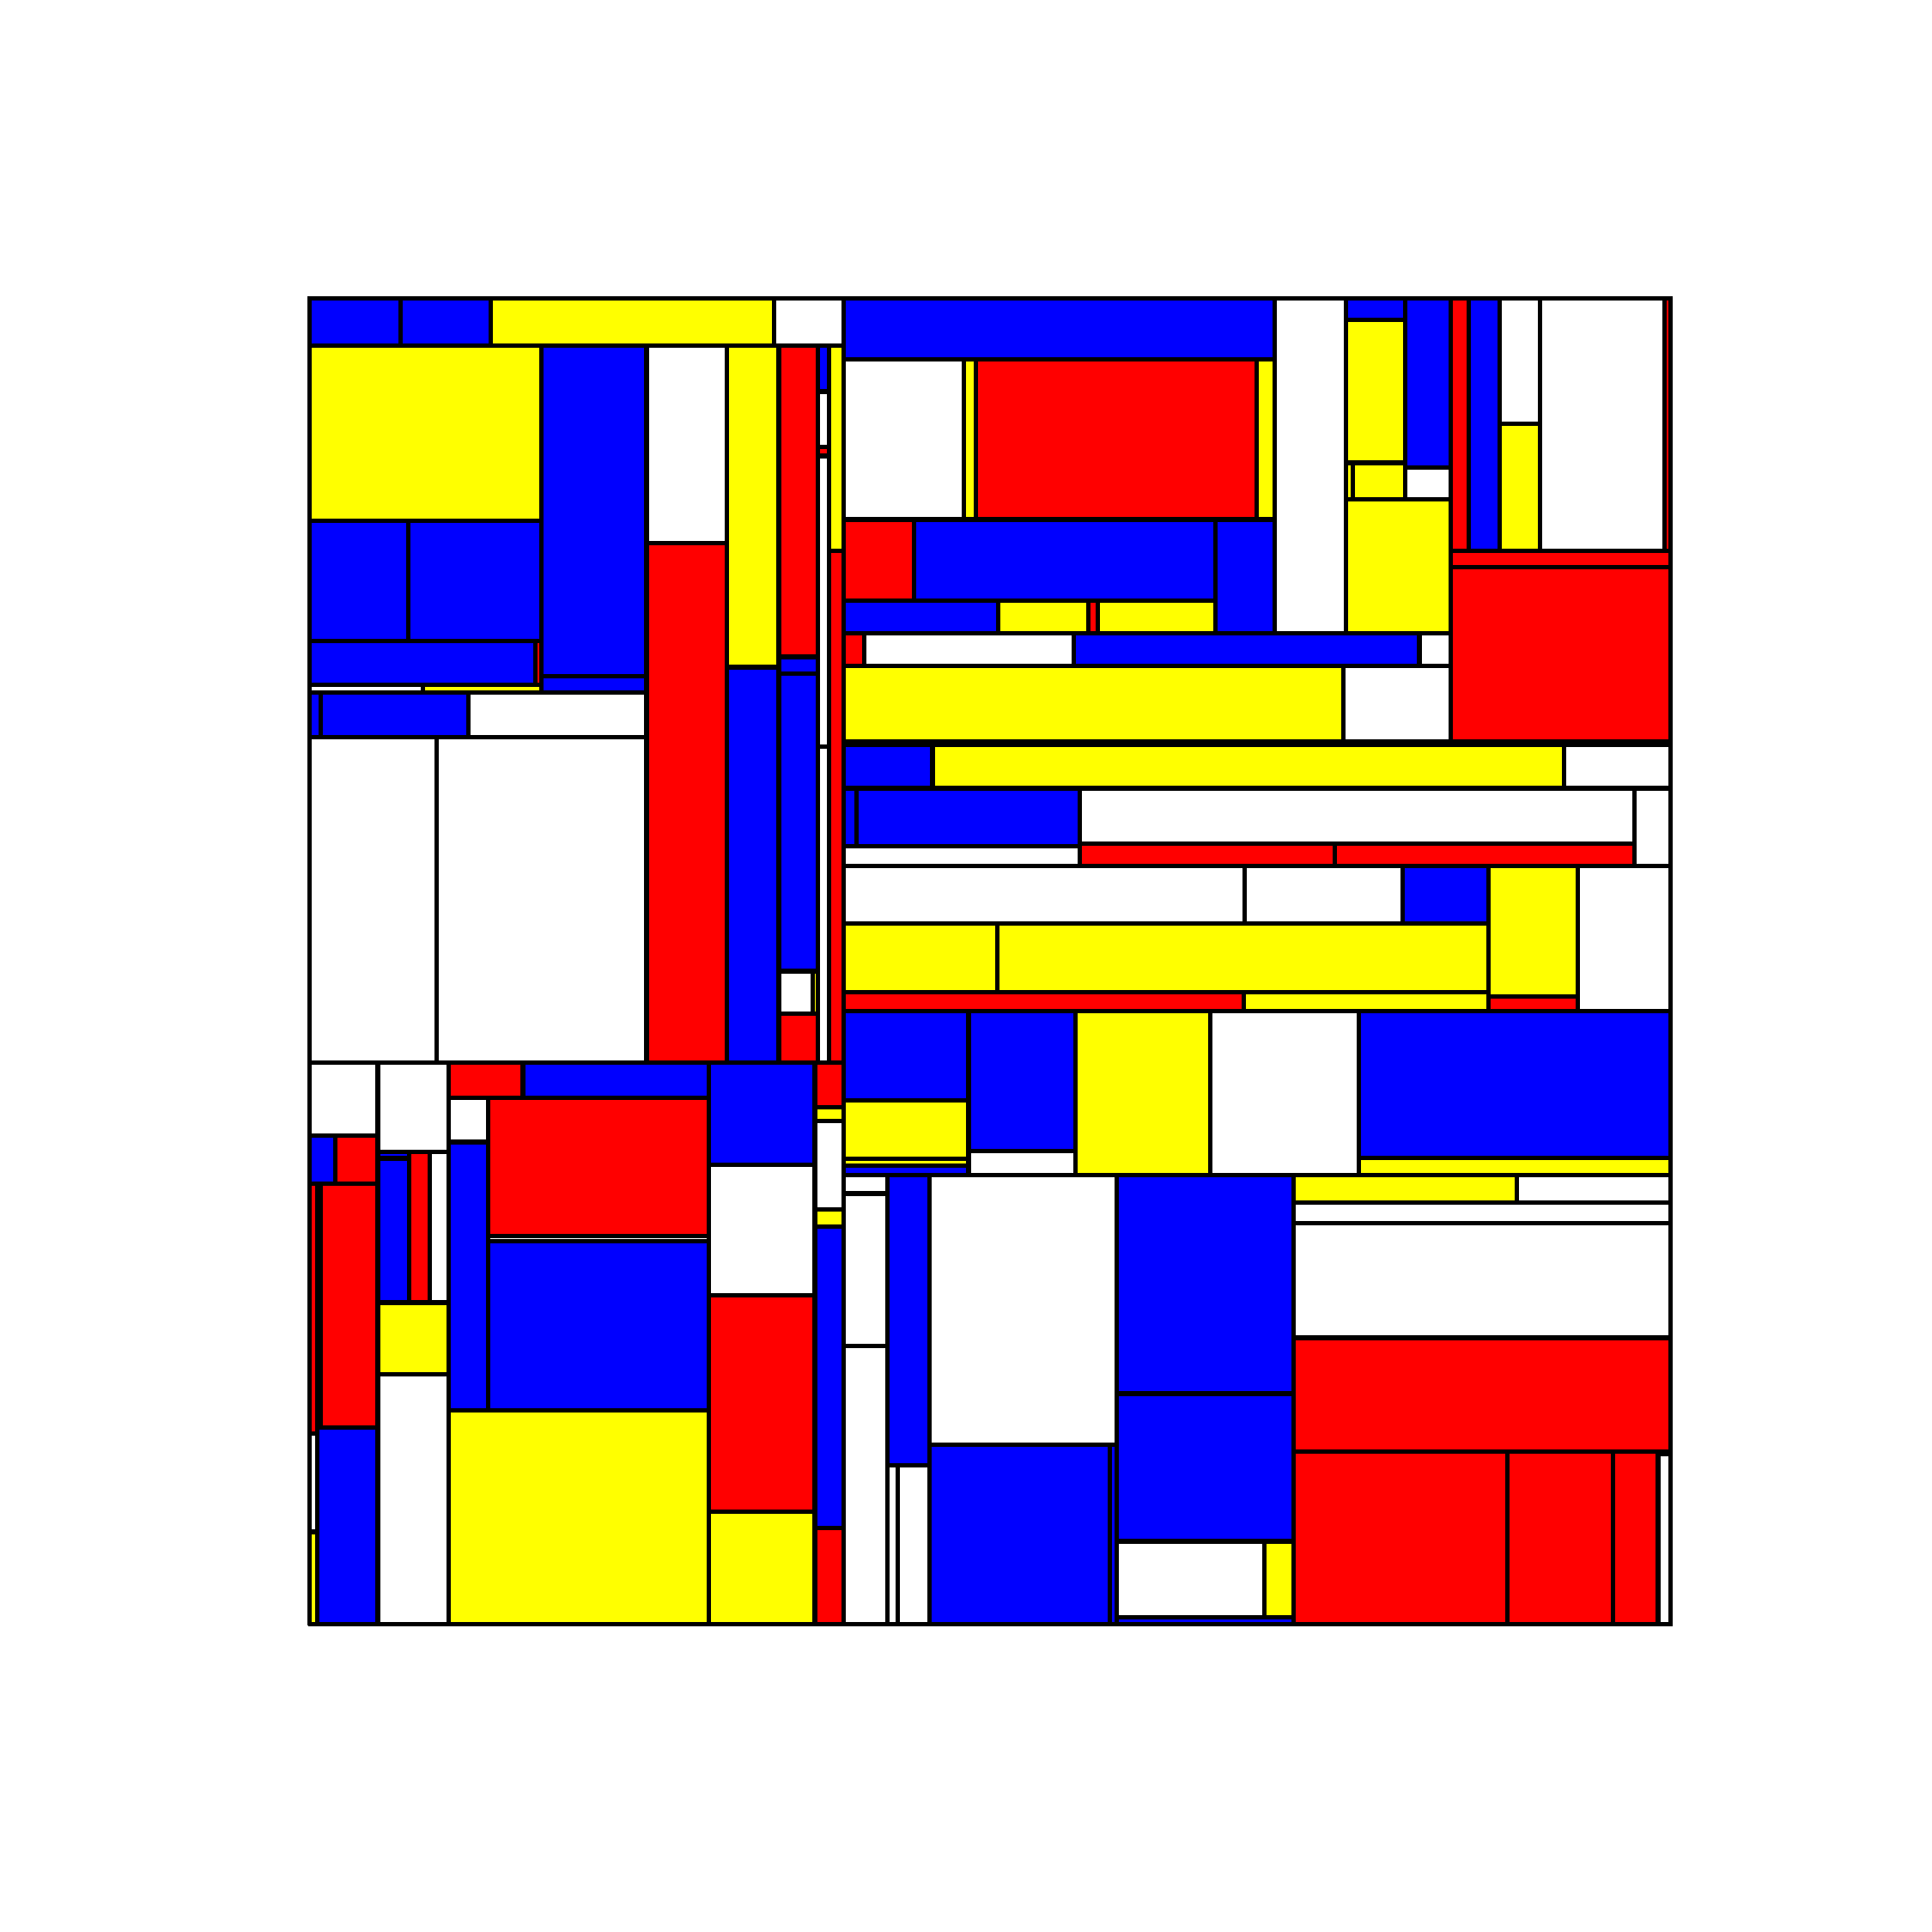
\includegraphics[width = \linewidth]{prebuiltimages/Mondrianbudget10.pdf}
  \end{subfigure}%
  \hspace{2em}% Space between image B and C
  \begin{subfigure}{.3\linewidth}
    \centering
    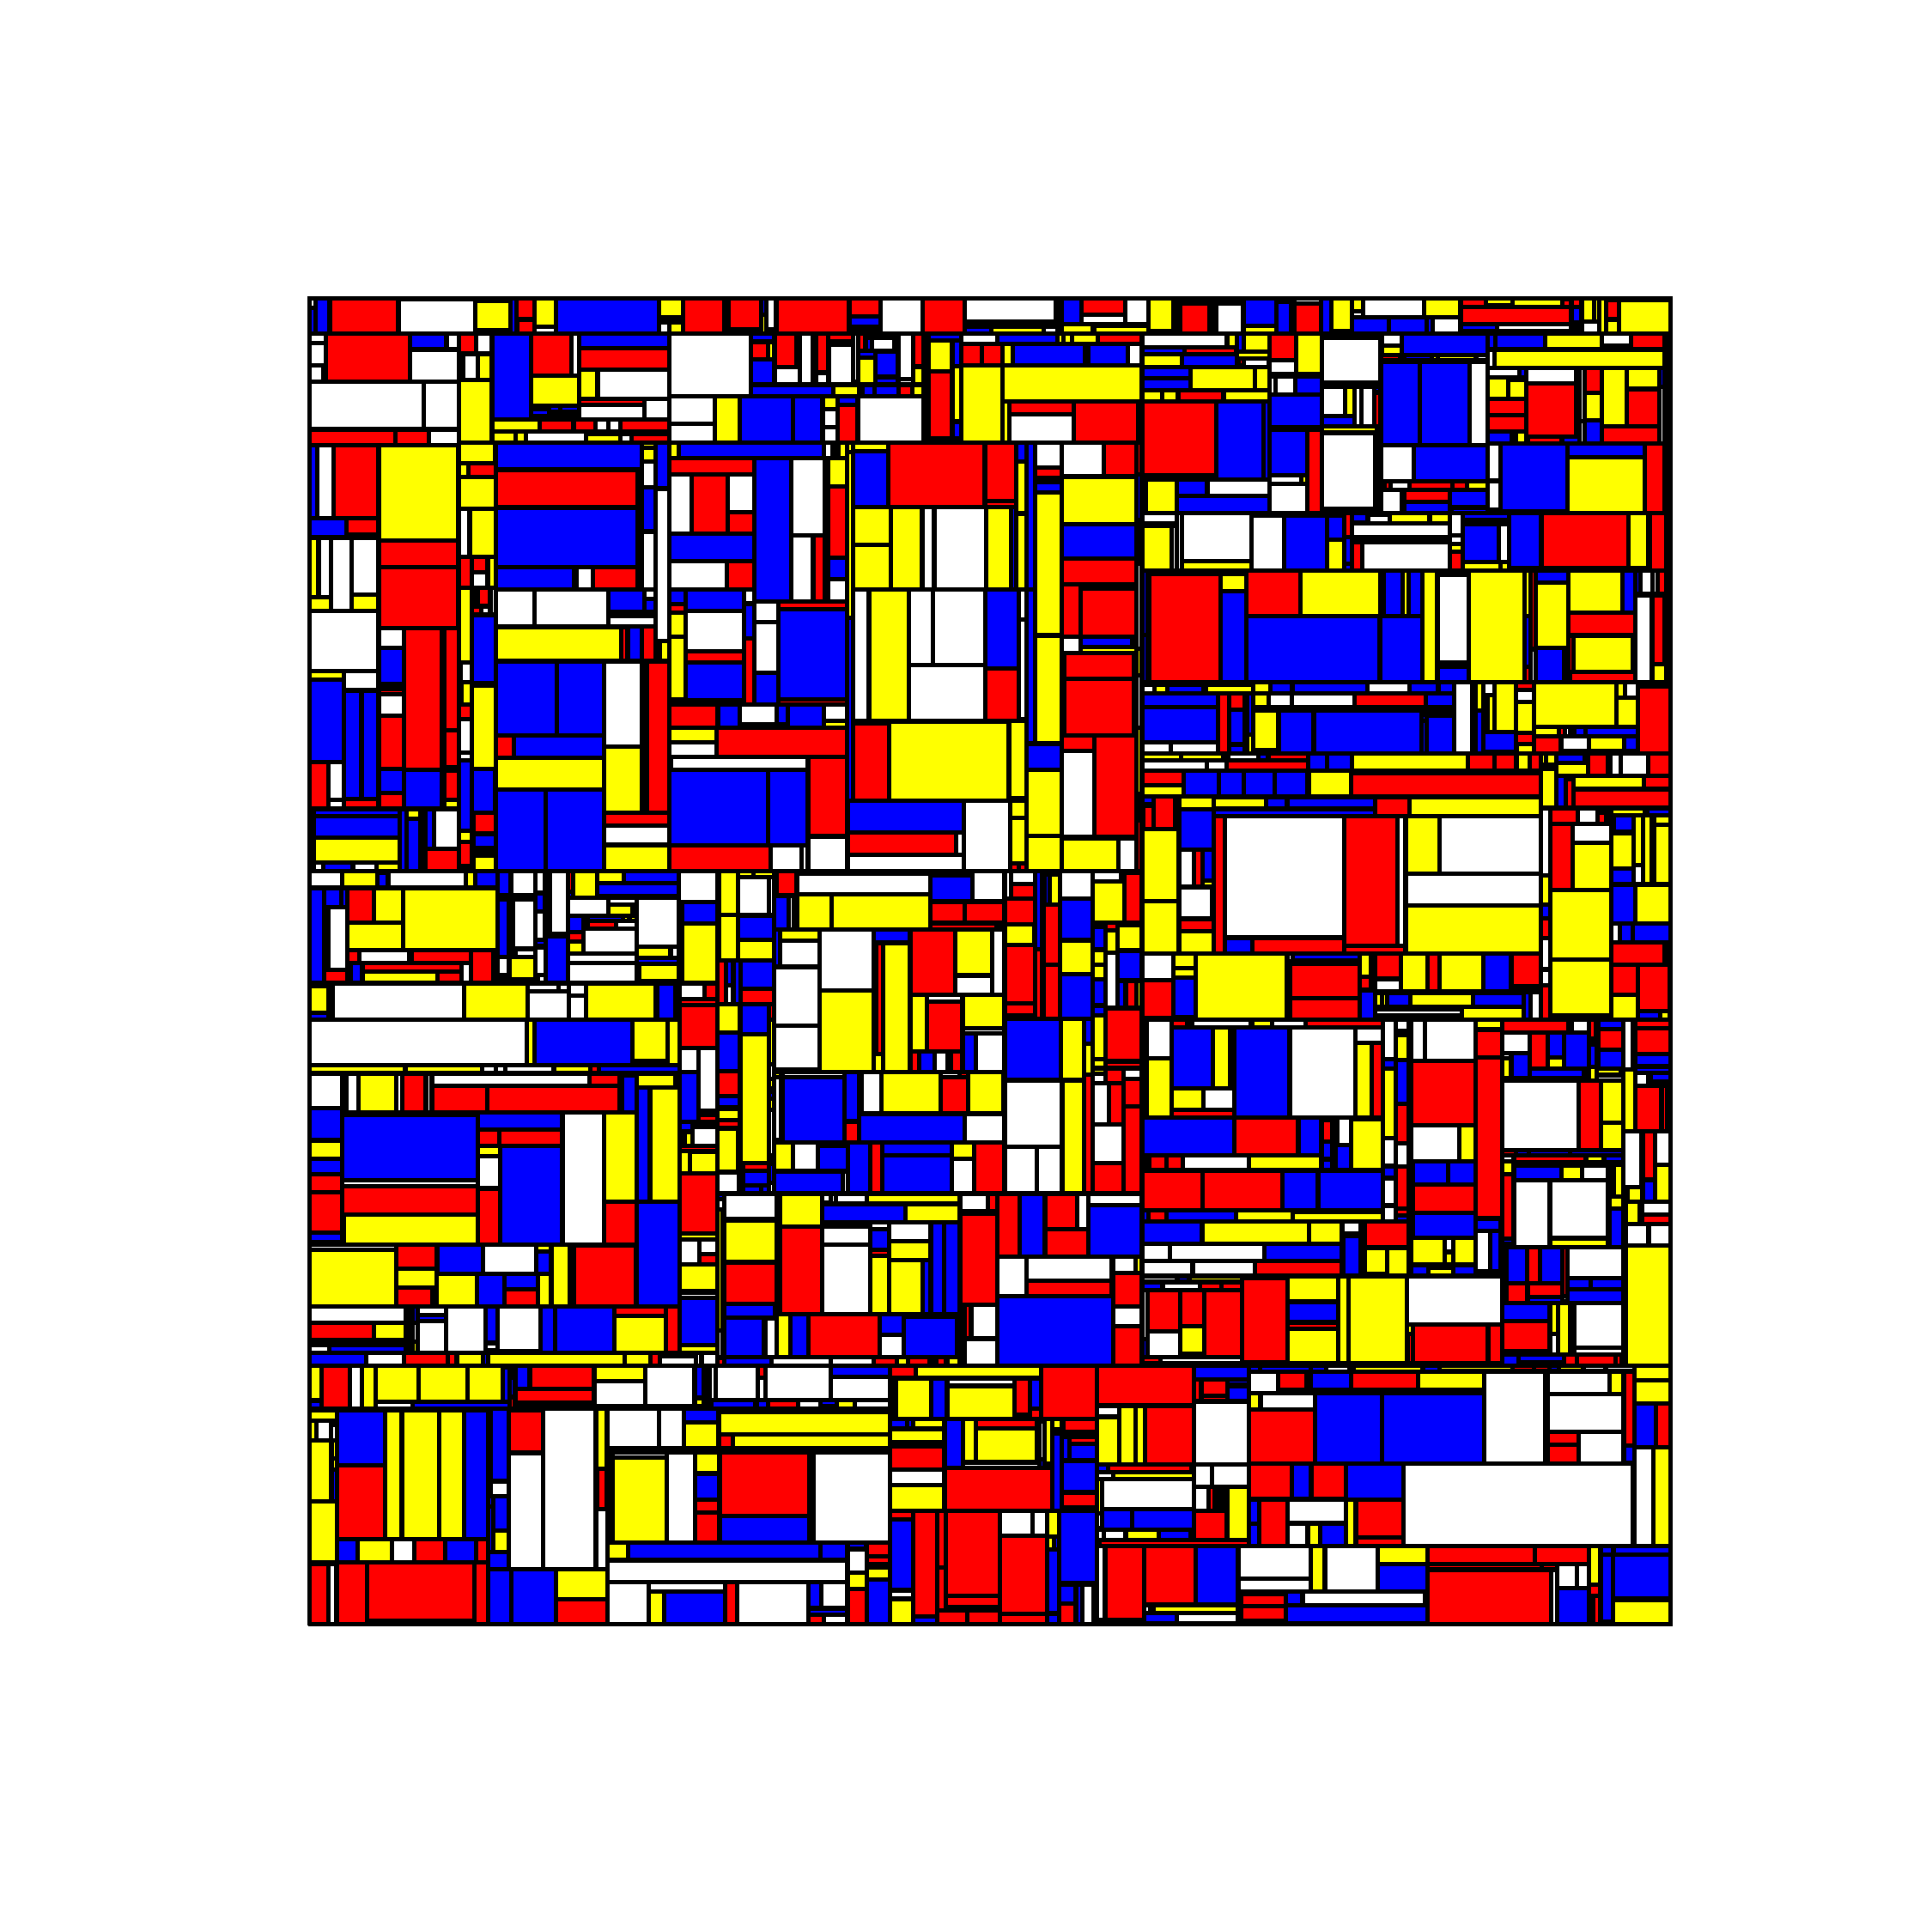
\includegraphics[width = \linewidth]{prebuiltimages/Mondrianbudget50.pdf}
  \end{subfigure}
  \caption{Exemple générateur aléatoire Mondrian (budget=2,10,50)}
\end{figure}


Ici on peut voir un fait intéressent a propos de ce générateur est que sur chaque coupe (division) les deux nouveaux blocs qui en résultent sont conditionnellement indépendants l'un de l'autre. 

\newpage

\subsection{Forêt Mondrian sur nos données DIGITS}
Dans cette partie, nous allons utilisé le jeu de données \textbf{"Boston Housing"}, il comprend le prix des maisons dans divers endroits de Boston. Outre le prix, l'ensemble de données fournit également des informations telles que la criminalité (CRIM), les zones d'activités non commerciales dans la ville (INDUS), l'âge des personnes qui possèdent la maison (AGE), et il existe de nombreux autres attributs.

\begin{center}
\begin{tabular}{ c c c c c c c c c c c c c c c}
\hline
CRIM & ZN & INDUS & CHAS & NOX & RM & AGE & DIS & RAD & TAX & PTRATIO & B & LSTAT\\
\hline
0.00632 & 18.0 & 2.31 & 0.0 & 0.538 & 6.575	& 65.2 & 4.0900	& 1.0 & 296.0 & 15.3 & 396.90 & 4.98\\
0.02731 & 00.0 & 7.07 & 0.0 & 0.469	& 6.421	& 78.9 & 4.9671	& 2.0 & 242.0 & 17.8 & 396.90 & 9.14\\
0.02729 & 00.0 & 7.07 & 0.0 & 0.469	& 7.185	& 61.1 & 4.9671	& 2.0 & 242.0 & 17.8 & 392.83 & 4.03\\
0.03237 & 00.0 & 2.18 & 0.0 & 0.458	& 6.998	& 45.8 & 6.0622	& 3.0 & 222.0 & 18.7 & 394.63 & 2.94\\
0.06905 & 00.0 & 2.18 & 0.0 & 0.458	& 7.147	& 54.2 & 6.0622	& 3.0 & 222.0 & 18.7 & 396.90 & 5.33\\
\hline
\end{tabular}
\end{center}

\begin{itemize}
    \item[$\bullet$] \textbf{CRIM:} taux de criminalité par habitant par ville
    \item[$\bullet$] \textbf{ZN:} proportion de terrains résidentiels zonés pour les lots de plus de $25 000 m^2$
    \item[$\bullet$] \textbf{INDUS:} proportion d'acres non commerciales par ville
    \item[$\bullet$] \textbf{CHAS:} Variable fictive de Charles River ($1$ si la zone délimite la rivière, $0$ sinon)
    \item[$\bullet$] \textbf{NOX:} concentration d'oxydes nitriques (parties par $10$ millions)
    \item[$\bullet$] \textbf{RM:} nombre moyen de pièces par logement
    \item[$\bullet$] \textbf{AGE:} proportion de logements occupés par leur propriétaire construits avant 1940
    \item[$\bullet$] \textbf{DIS:} distances pondérées jusqu'à cinq centres d'emploi de Boston
    \item[$\bullet$] \textbf{RAD:} indice d'accessibilité aux autoroutes (radiales)
    \item[$\bullet$] \textbf{TAX:} taux d'imposition foncière de la valeur totale par tranche de 10000 \$
    \item[$\bullet$] \textbf{PTRATIO:} ratio élèves-enseignant par ville
    \item[$\bullet$] \textbf{B:} $1000 (Bk - 0,63) ^ 2$ où $Bk$ est la proportion d'afro américains par ville
    \item[$\bullet$] \textbf{LSTAT:} \% statut inférieur de la population
    \item[$\bullet$] \textbf{MEDV:} Valeur médiane des logements occupés par leur propriétaire en milliers de dollars
\end{itemize}

\begin{figure}[H]
  \centering
  \begin{subfigure}{.3\linewidth}
    \centering
    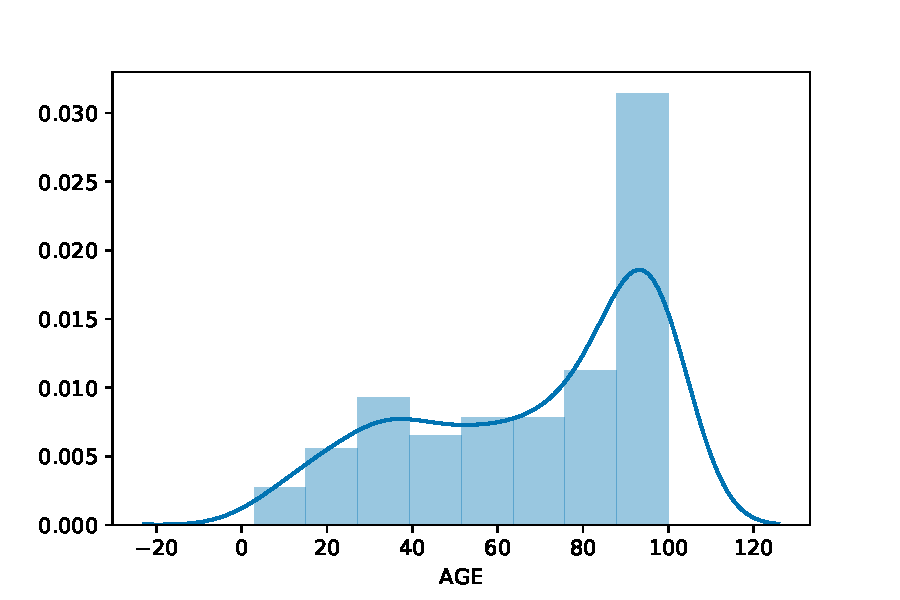
\includegraphics[width = \linewidth]{prebuiltimages/Age.pdf}
    \caption{Logement occupé construit < 1940}
  \end{subfigure}%
  \hspace{1em}% Space between image A and B
  \begin{subfigure}{.3\linewidth}
    \centering
    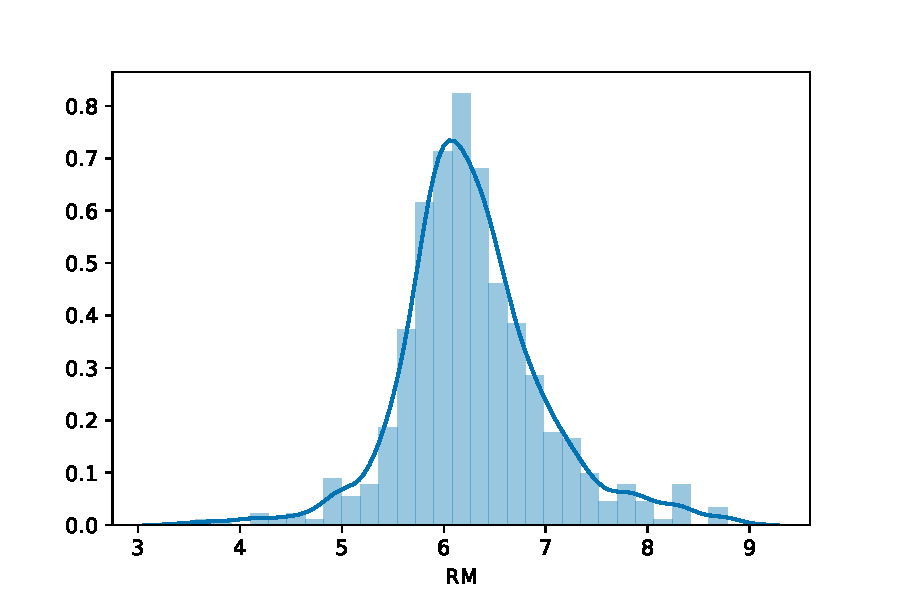
\includegraphics[width = \linewidth]{prebuiltimages/RM.pdf}
    \caption{Nombre pièces}
  \end{subfigure}%
  \hspace{2em}% Space between image B and C
  \begin{subfigure}{.3\linewidth}
    \centering
    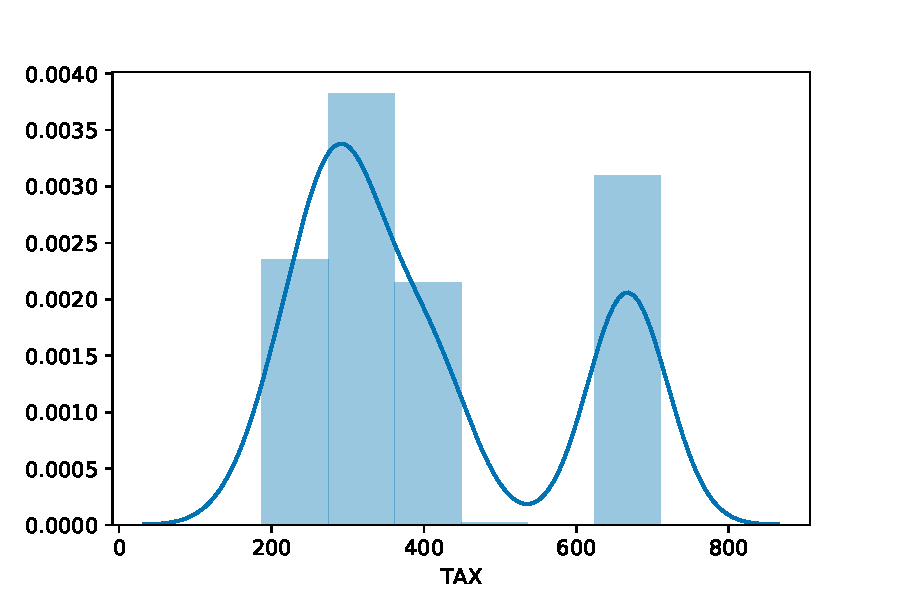
\includegraphics[width = \linewidth]{prebuiltimages/TAX.pdf}
    \caption{Taux d'imposition}
  \end{subfigure}
  \caption{Représentation graphique de quelques variables}
\end{figure}

A l'aide du package "$skgarden$" il nous ait possible d'importer les fonction "$MondrianForestCLassifier$", "$MondrianForestRegressor$",
"$MondrianTreeClassifier$" et
"$MondrianTreeRegressor$"

\newpage

\section{Conclusion}
Nous avons introduit les forêts de Mondrian, une nouvelle classe de forêts aléatoires qui est une notion nouvelle et récente. Nous avons aussi dans ce projet créer une fonction génératrice qui nous permet de simuler et de mieux voir la méthode de fonctionnement des forêts de Mondrian. 


\begin{thebibliography}{99}
\bibitem{1} Mondrian Forests: Efficient Online Random Forests\\
{\it Balaji Lakshminarayanan (University College London), Daniel M. Roy (University of Cambridge),Yee Whye Teh(Department of Statistics University of Oxford)}
\end{thebibliography}

\newpage
